\section{Mechanical Design}

Our initial criteria for the mechanical design of the robot were as follows:
\begin{itemize}
    \item Slightly larger than 2' x 3' frame.
    \item Tall point at rear for camera, with drive wheels in view.
    \item As near to zero-point turning as reasonable.
    \item LiDAR directly over center of drive axle.
    \item Main weight (battery, payload) positioned over or between the axles.
\end{itemize}

We decided to use a triangular wedge shape for the chassis for many reasons; the center of mass is moved further back, which allows us to shift the drive wheels towards the center without the threat of tipping forward. This also helps the camera to be able to see the drive wheels, which allows us on the software end to see if we're in the lanes easily.

% \begin{figure}[h]
% \begin{tabular}{ll}
% 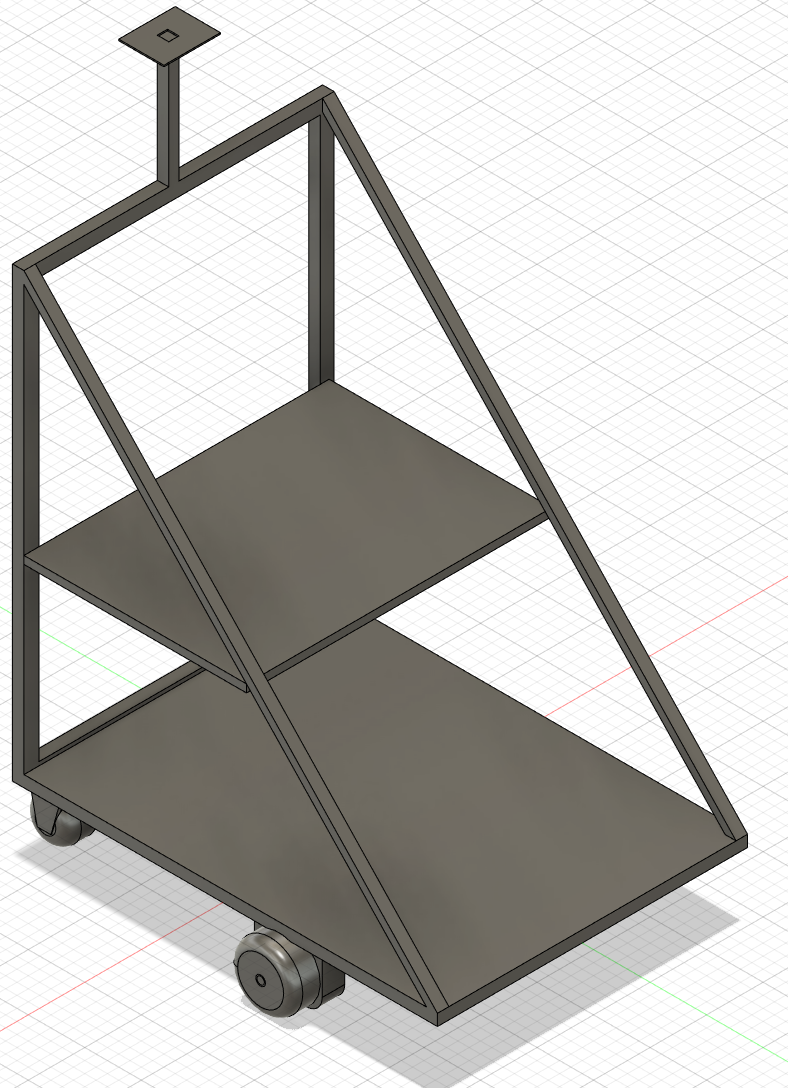
\includegraphics[scale=0.04]{images/frame/frame2.PNG}
% &
% 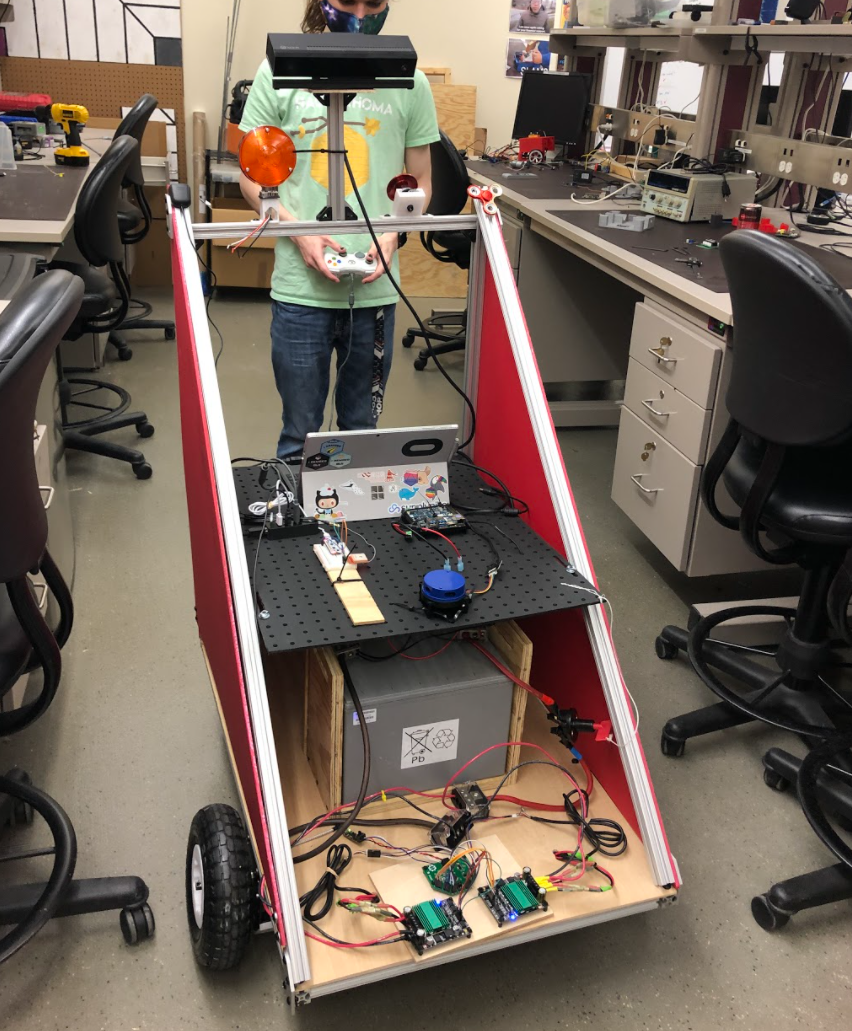
\includegraphics[scale=0.04]{images/frame/real.JPG}
% \end{tabular}
% \caption{The basic structure of the robot.}
% \end{figure}

\begin{figure}[h]
  \centering
  \begin{minipage}[b]{0.35\textwidth}
    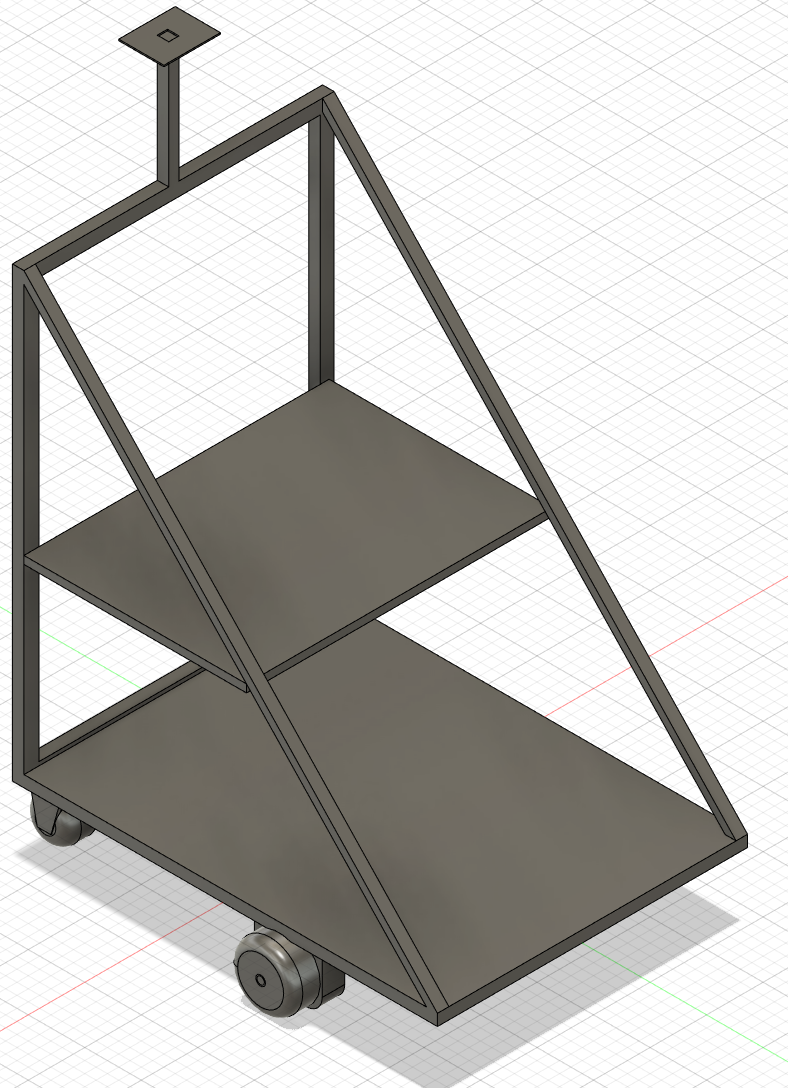
\includegraphics[width=\textwidth]{images/frame/frame2.PNG}
    \caption{CAD model for the basic structure.}
  \end{minipage}
  \hfill
  \begin{minipage}[b]{0.4\textwidth}
    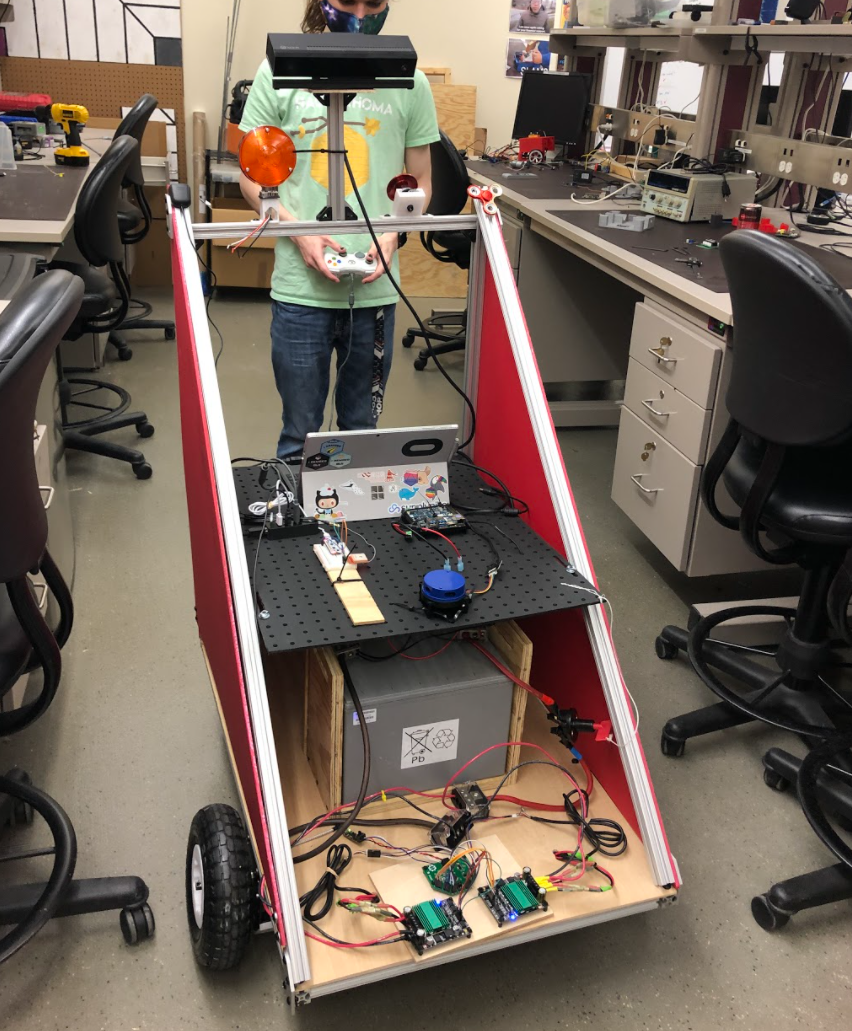
\includegraphics[width=\textwidth]{images/frame/real.PNG}
    \caption{Physical robot with most components installed.}
  \end{minipage}
\end{figure}

% \begin{figure}[h]
%     \centering
%     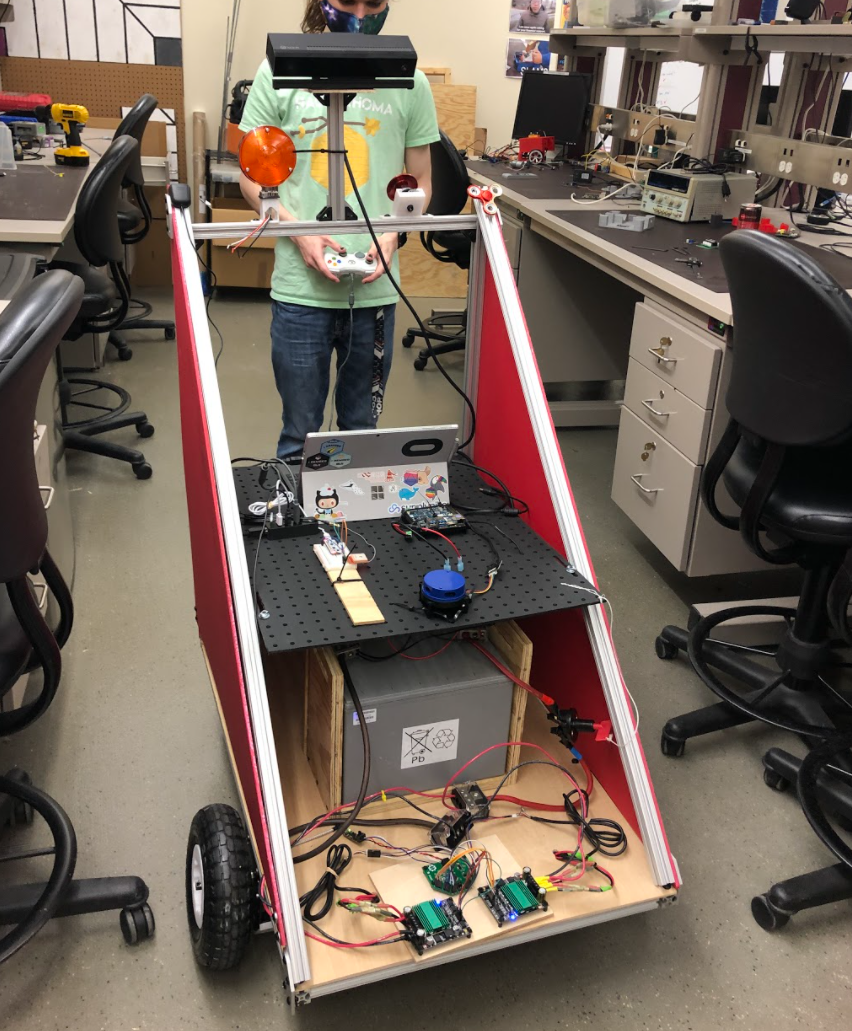
\includegraphics[width=0.4\textwidth]{images/frame/real.PNG}
%     \caption{Basic aluminum frame of the robot, with a wooden base panel, polyboard shelf for the electronics, and red acrylic paneling on the sides.}
% \end{figure}

The basic frame of the robot is composed of aluminum T-slot channels in two triangles connected at the three vertices, with additional support trusses on the underside. The base of the robot is a wooden panel supported underneath by several aluminum channels. On these channels are mounted two casters at the back corners and the two gearboxes about 2/3 of the way up the robot. We decided on this position as a good balance between perfect zero-point turns (wheels at midpoint) and the most usable space on the robot for heavy payloads (wheels at the front). We position our heavy robot battery on the wooden base directly over the drive axle and load the cinder block behind it, between the two ``axles''.

We've mounted a polyboard shelf 15" above the wooden base, which we use to attach most electronics. This height was chosen to give a few inches of clearance above our battery box. The holes in the polyboard are helpful for wire and cable routing, and there are more significant gaps at the sides for connectors too big for the holes. This shelf sticks out 5" beyond the aluminum slant to mount the LiDAR above the drive axle with as little obstruction as possible. This gives us near 180 degrees LiDAR data. The LiDAR mount is shown in FIG. \ref{fig:mount:lidar}.

\begin{figure}[h]
    \centering
    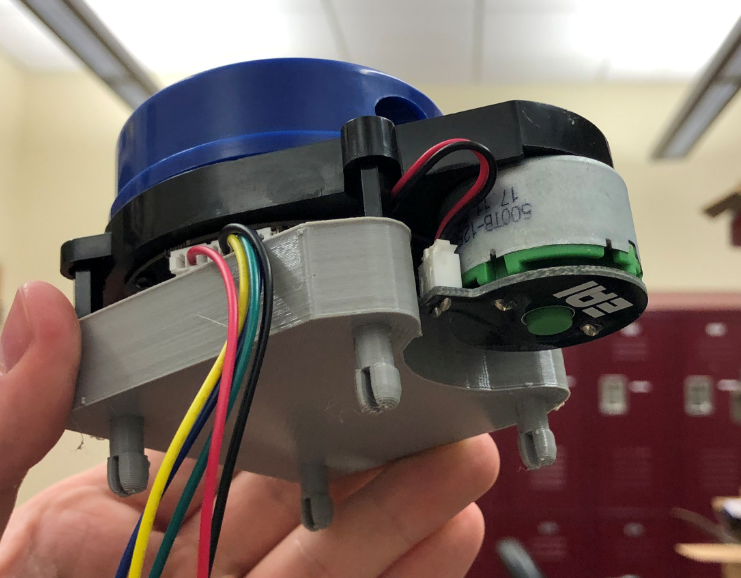
\includegraphics[width=0.4\textwidth]{images/lidar_mount.PNG}
    \caption{3D printed LiDAR mount easily attaches to the polyboard shelf.}
    \label{fig:mount:lidar}
\end{figure}

The camera we're using is the X-Box Kinect 2, which is mounted at the top of the tall pole at the rear of our robot to give it the best view. We mount it onto a small flat piece of wood to improve stability.

We have no formal suspension, opting for flexible mounting of components and built-in tolerance in code for shaky camera and LiDAR data.

The weatherproofing plan consists of enclosing the chassis by acrylic panels on all sides, with caulk or foam filling the gaps. Our concerns with fully enclosing the robot include accessibility to components for maintenance and heating inside the chassis. We subvert this first issue by including hinged panels on areas that will need access, and designing the layout of the components within the robot to be centralized to these such areas. All electronics are located on the shelf midway up the robot with the exception of the motor controllers, which are at the very front of the robot. This means we could ensure everything is accessible from the slanted front face when it is open.

\begin{figure}[h]
    \centering
    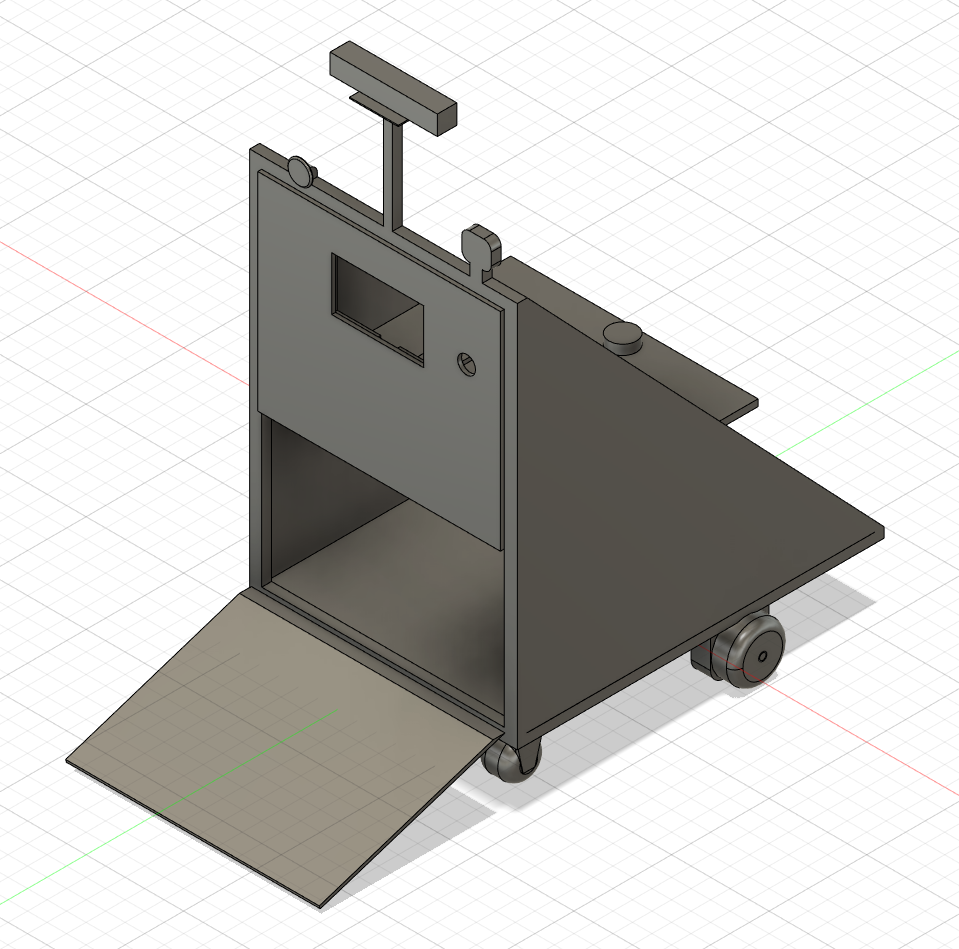
\includegraphics[width=0.5\textwidth]{images/frame/frame5.PNG}
    \caption{The lower-back panel hinges open to provide a loading point for the robot battery and the cinder block payload. The rectangular gap on the upper part is for a screen that shows debug information while the robot runs.}
\end{figure}

To help with air circulation inside the robot, we leave some small downward-facing gaps near the upper part of the robot, which lets air passively circulate with minimal danger of rainfall entering. We do not believe active cooling (i.e., with fans) is necessary for our setup. Since we need to partially disassemble the robot for our travel to and from the competition, we will bring the caulk and, only if necessary, apply it to gaps between paneling on the lower part of the robot, and seal wire-access holes on the base with caulk or hot glue. We aren't worried about water entry through the lower-rear hinged panel since it will be adjacent to the cinder block and not very close to any electronics. 

The main concern for waterproofing with our sleek design is the LiDAR. It needs to be accessible to the open air and cannot be surrounded by plexiglass, plastic, or even saran wrap. We have designed a covering to be installed directly over it to be used for light rain, but if the weather worsens, we will be removing the LiDAR for its safety. As will be discussed in later sections, our robot can function even if individual modules are removed. Our software is robust with multiple different input sources, so it will still perform without LiDAR data.